\documentclass{article}

\usepackage{fancyhdr} % Required for custom headers
\usepackage{lastpage} % Required to determine the last page for the footer
\usepackage{amsmath}
\usepackage{amsfonts}
\usepackage{dsfont}
\usepackage{graphicx}
\usepackage{subfigure}
\usepackage{listings}
\usepackage{booktabs}
\usepackage[hidelinks]{hyperref}
% \usepackage{epstopdf} uncomment this line if using MiKTeX

% Margins
\topmargin=-0.45in
\evensidemargin=0in
\oddsidemargin=0in
\textwidth=6.5in
\textheight=9.0in
\headsep=0.25in

\linespread{1.25} % Line spacing

% Set up the header and footer
\pagestyle{fancy}
\lhead{\authorName} % Top left header
\chead{\classID\ \hwTitle} % Top center header
\rhead{\studentID} % Top right header
\lfoot{} % Bottom left footer
\cfoot{} % Bottom center footer
\rfoot{Page\ \thepage\ of~\pageref{LastPage}} % Bottom right footer
\renewcommand{\headrulewidth}{0.4pt} % Size of the header rule
\renewcommand{\footrulewidth}{0.4pt} % Size of the footer rule

\setlength{\parindent}{0pt} % Removes all indentation from paragraphs

\setcounter{secnumdepth}{0} % Removes default section numbers
\newcounter{problemCounter} % Creates a counter to keep track of the number of problems

\newcommand{\problemName}{}
\newenvironment{problem}[1][Problem \arabic{problemCounter}]{
	\stepcounter{problemCounter} % Increase counter for number of problems
	\renewcommand{\problemName}{#1} % Assign \problemName the name of the problem
	\section{\problemName} % Make a section in the document with the custom problem count
}{}

\newcommand{\subproblemName}{}
	\newenvironment{subproblem}[1]{
	\renewcommand{\subproblemName}{#1} % Assign \subproblemName to the name of the section from the environment argument
	\subsection{\subproblemName} % Make a subsection with the custom name of the subsection
}{}

%----------------------------------------------------------------------------------------
%	MATH OPERATOR
%----------------------------------------------------------------------------------------

\DeclareMathOperator*{\argmin}{arg\,min}
\DeclareMathOperator*{\argmax}{arg\,max}

%----------------------------------------------------------------------------------------
%	NAME AND CLASS SECTION
%----------------------------------------------------------------------------------------

\newcommand{\hwTitle}{Assignment\ \#2} % Assignment title
\newcommand{\dueDate}{Thursday,\ March\ 21,\ 2017} % Due date
\newcommand{\classID}{ELEG\ 5491} % Course/Class
\newcommand{\authorName}{Kai Chen} % Your name
\newcommand{\studentID}{1155070509} % Your student ID

%----------------------------------------------------------------------------------------
%	TITLE PAGE
%----------------------------------------------------------------------------------------

\title{
	\vspace{2in}
	\textmd{\textbf{\classID:\ \hwTitle}}\\
	\normalsize\vspace{0.1in}\small{Due\ on\ \dueDate}
	\vspace{3in}
}

\author{\textbf{\authorName}}
\date{} % Insert date here if you want it to appear below your name

%----------------------------------------------------------------------------------------

\begin{document}
\maketitle
\setcounter{page}{0}
\thispagestyle{empty}
\newpage

%----------------------------------------------------------------------------------------
%	PROBLEM 1
%----------------------------------------------------------------------------------------

% To have just one problem per page, simply put a \clearpage after each problem

\begin{problem}

\begin{align*}
\frac{\partial L}{\partial W_{hz}} &= \frac{\partial \sum_t -\log z_{t, y_t}}{\partial W_{hz}} \\
&= -\sum_t \frac{1}{z_{t, y_t}} \frac{\partial z_{t, y_t}}{\partial W_{hz}}
\end{align*}
Let $o_t = W_{hz}h_t + b_z$, then
\begin{align*}
\frac{\partial z_{t, y_t}}{\partial W_{hz}} &= \frac{\partial z_{t, y_t}}{\partial o_t} \frac{\partial o_t}{\partial W_{hz}} \\
&= \begin{cases}
-z_{t, y_t}z_{t, i}h_t, & \text{if } i \neq y_t \\
z_{t, y_t}(1 - z_{t, i})h_t, & \text{if } i = y_t
\end{cases} \\
&= z_{t, y_t}h_t(\delta^i_{y_t} - z_t)^T \\
%&= z_{t, y_t}
%\begin{bmatrix}
%z_{t,1}h_t, & z_{t,2}h_t, & \dots, & (1-z_{t, y_t})h_t, & \dots, & z_{t,n}h_t
%\end{bmatrix}
\end{align*}
where 
\[
\delta^i_j=
\begin{cases}
1, & \text{if } i = j \\
0, & \text{if } i \neq j
\end{cases}
\]
So
\begin{align*}
\frac{\partial L}{\partial W_{hz}} &= -\sum_t \frac{1}{z_{t, y_t}} \frac{\partial z_{t, y_t}}{\partial W_{hz}} \\
&= \sum_t h_t(z_t - \delta^i_{y_t})^T
%\begin{bmatrix}
%z_{t,1}h_t, & z_{t,2}h_t, & \dots, & (z_{t, y_t} - 1)h_t, & \dots, & z_{t,n}h_t
%\end{bmatrix}
\end{align*}

\begin{align*}
\frac{\partial L}{\partial W_{hh}} &= \frac{\partial L}{\partial h_t} \frac{\partial h_t}{\partial W_{hh}} \\
&= (\frac{\partial L}{\partial h_{t+1}} \frac{\partial h_{t+1}}{\partial h_t} + \frac{\partial L}{\partial z_t} \frac{\partial z_t}{\partial h_t})\frac{\partial h_t}{\partial W_{hh}} \\
&= (\frac{\partial L_{t+1}}{\partial z_{t+1}} \frac{\partial z_{t+1}}{\partial h_{t+1}} \frac{\partial h_{t+1}}{\partial h_t} + \frac{\partial L_t}{\partial z_t} \frac{\partial z_t}{\partial h_t})\frac{\partial h_t}{\partial W_{hh}} \\
&= (W_{hz}^T(z_{t+1}-\delta^i_{y_{t+1}})W_{hh}(1-h_{t+1}^2)+W_{hz}^T(z_t-\delta^i_{y_t}))(1-h_t^2)h_{t-1}
\end{align*}

\end{problem}

%----------------------------------------------------------------------------------------
%	PROBLEM 2
%----------------------------------------------------------------------------------------

\begin{problem}

\begin{subproblem}{2.1}

\begin{align*}
h_t &= G_t(x_t, \dots, x_1) \\
&= F_\theta(h_{t-1}, x_t) \\
&= F_\theta(F_\theta(h_{t-2}, x_{t-1}), x_t) \\
&= \dots
\end{align*}
	
\end{subproblem}

\begin{subproblem}{2.2}

1. The RNN units share parameters among different time steps.

2. The current \(h_t\) contains information about the whole past sequence.

\end{subproblem}


\end{problem}

%----------------------------------------------------------------------------------------
%	PROBLEM 3
%----------------------------------------------------------------------------------------

\begin{problem}

At stage 3, 6 and 7.

\end{problem}

%----------------------------------------------------------------------------------------
%	PROBLEM 4
%----------------------------------------------------------------------------------------

\begin{problem}

	
\begin{subproblem}{4.1}

\(dn+(L-1)n^2+nc\)
	
\end{subproblem}

\begin{subproblem}{4.2}

Forward: \(dn+(L-1)n^2+nc\)

Backward: \(2(dn+(L-1)n^2+nc)\)

Total: \(O(dn+(L-1)n^2+nc) = O((c+d+Ln)n)\)

\end{subproblem}

\begin{subproblem}{4.3}

Backward: \(
2nc + 2n^2(c+2cn+,\dots,+Lcn^{L-1}) + 2nd((L+1)cn^L) = O(cdLn^{L+1})
\)
	
\end{subproblem}

\end{problem}

%----------------------------------------------------------------------------------------
%	PROBLEM 5
%----------------------------------------------------------------------------------------

\begin{problem}
	
\begin{subproblem}{5.1}
	
Training curve is shown in Fig.~\ref{fig:loss}, and the filters learned in the first convolutional layer is shown in Fig.~\ref{fig:filter}. The test accuracy is 63.4\%(with weight decay of $0.0005$) and 61.2\%(without weight decay).
\begin{figure}[htbp]
	\begin{center}
		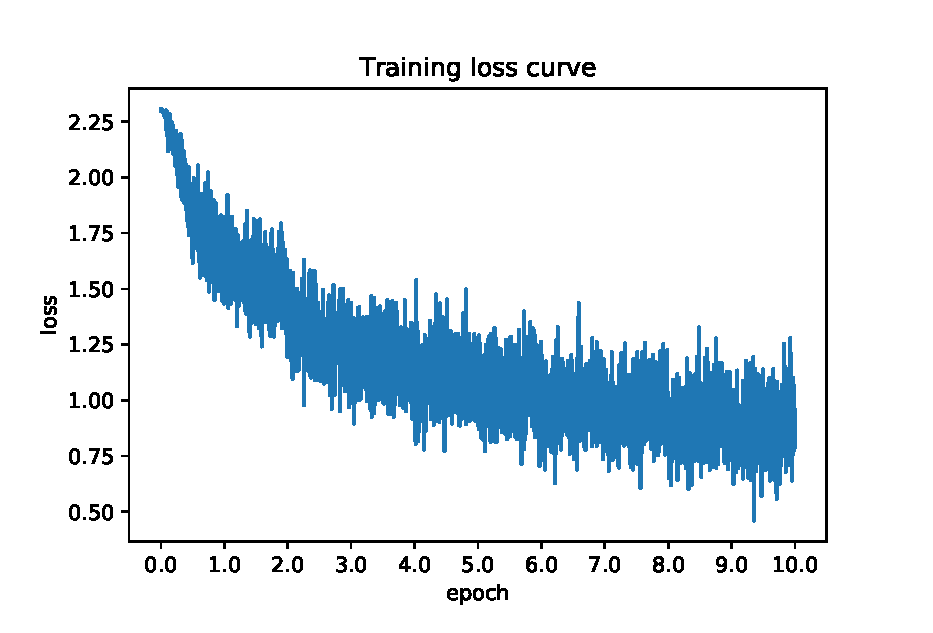
\includegraphics[width=0.6\linewidth]{image/loss.eps}
	\end{center}
	\caption{Training curve.}
	\label{fig:loss}
\end{figure}

\begin{figure}[htbp]
	\begin{center}
		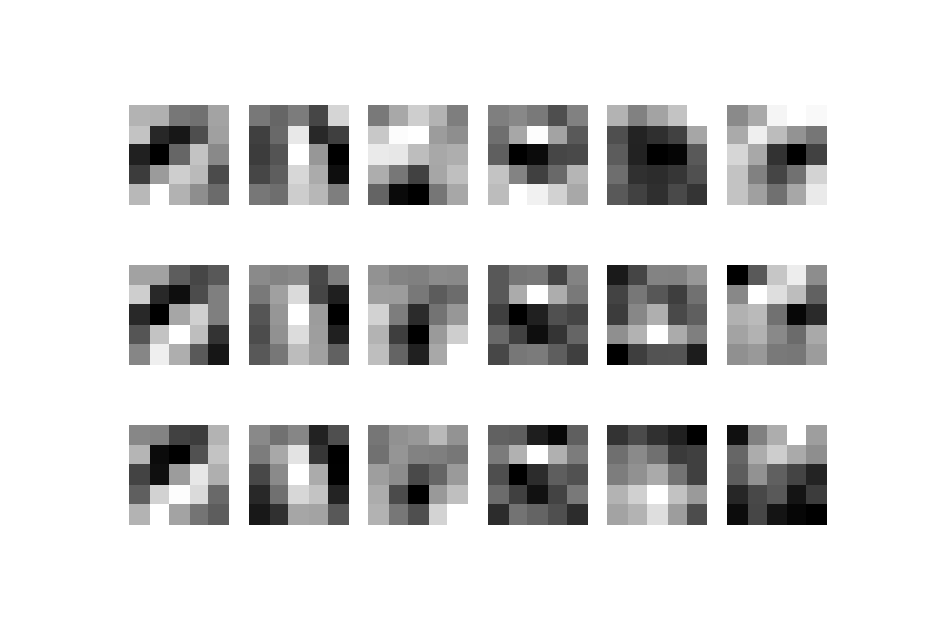
\includegraphics[width=0.6\linewidth]{image/filters.eps}
	\end{center}
	\caption{Visualization of filters.}
	\label{fig:filter}
\end{figure}
	
\end{subproblem}

\begin{subproblem}{5.2}

Proof of equation 3 and 4 is as following.
\begin{align*}
Var[y_l] &= n_lVar[w_lx_l] \\
&= n_l (E^2[w_l]Var[x_l] + E^2[x_l]Var[w_l] + Var[x_l]Var[w_l]) \\
&= n_l (E^2[x_l]Var[w_l] + Var[x_l]Var[w_l]) \\
&= n_l Var[w_l](E^2[x_l] + Var[x_l]) \\
&= n_l Var[w_l] E[x^2_l]
\end{align*}

\begin{align*}
E[x^2_l] &= \int_{-\infty}^{+\infty}[ReLU(y_{l-1})]^2p(y)dy \\
&= \int_0^{+\infty}y^2_{l-1}p(y)dy \\
&= \frac{1}{2}\int_{-\infty}^{+\infty}y^2_{l-1}p(y)dy \\
&= \frac{1}{2}\int_{-\infty}^{+\infty}(y - E[y_{l-1}])^2p(y)dy \\
&= \frac{1}{2}Var[y_{l-1}]
\end{align*}

The test accuracy is 64.1\% compared with 63.4\% in result 1.

\end{subproblem}

\begin{subproblem}{5.3}

Adding BN layers and increasing batch size to 32 boosts the test accuracy to 65.6\%.
	
\end{subproblem}

\end{problem}


\end{document}
